%% Elsevier CAS single-column manuscript
\documentclass[a4paper,fleqn]{cas-sc}
\usepackage[numbers,sort&compress]{natbib}
\usepackage{amsmath,amssymb,booktabs,graphicx,caption,float,placeins,xcolor,tikz,pgfplots}
\pgfplotsset{compat=1.18}
\usetikzlibrary{arrows.meta,positioning}
\newcommand{\E}{\mathbb{E}}
\newcommand{\FOM}{\mathrm{FOM}}
\newcommand{\WE}{\mathrm{WE}}
\begin{document}
\let\WriteBookmarks\relax
\def\floatpagepagefraction{1}
\def\textpagefraction{.001}

\shorttitle{Adjoint-Guided Rare-Event Sampling in Spin Systems}
\shortauthors{M.Y. Alzaatreh}
\title[mode=title]{Adjoint-Guided Rare-Event Sampling in Spin Systems: Weighted Ensembles and Learned Importance Coordinates}
\author{M.Y. Alzaatreh}\cormark[1]
\ead{mzaatreh@fbsu.edu.sa}
\credit{Conceptualization, Methodology, Software, Formal analysis, Investigation, Visualization, Writing -- original draft, Writing -- review \& editing}
\affiliation{organization={Natural Sciences Unit, Fahad Bin Sultan University},city={Tabuk},country={Saudi Arabia}}
\cortext[1]{Corresponding author}

\begin{abstract}
Rare-event simulation requires sampling effort to be concentrated in configurations that contribute disproportionately to a target response. Classical radiation transport addresses this problem through adjoint importance functions and weight-window population control, while transition-path theory describes the corresponding event-conditioned object through the committor. This correspondence is used here as a constructive framework for rare-event sampling in the two-dimensional Ising ferromagnet and Edwards--Anderson spin glass. A solvable birth--death process verifies the zero-variance limit obtained with exact importance, and exact enumeration on a $4\times4$ lattice confirms that weight-conserving Weighted Ensemble (WE) resampling reproduces the target distribution under different binning coordinates. At matched spin-update cost, WE extends the $L=20$ Ising magnetization tail from the naive sampling floor near $5.9\times10^{-6}$ to $2.4\times10^{-7}$, a factor of approximately 24 in probability. For the frustrated spin glass, a self-consistency-trained neural importance coordinate uses the full spin configuration to organize the weighted population. At the deepest calibrated target, pooled across three independent disorder realizations with one trained network each, the event is observed in $63/90$ learned-coordinate replicas against $46/90$ using the physical energy coordinate (70.0\% versus 51.1\%, Fisher exact $p=0.014$); a complementary check pooling three independently trained networks on a single realization against a matched-size baseline gives $60/90$ against $44/90$ (66.7\% versus 48.9\%, $p=0.023$). This reliability advantage does not translate into a wall-clock efficiency gain: repeated neural inference costs four to five times the wall-clock time of the energy coordinate, leaving a directly measured, bootstrapped figure of merit at roughly one-third of parity ($0.33$, 95\% CI $[0.19,0.58]$). These results establish a validated transport-theoretic route from exact adjoint importance to robust population control and learned configuration-space coordinates for sampling rare events in spin systems, with the reliability advantage reproduced across independent disorder realizations even though the corresponding efficiency gain is not yet realized.
\end{abstract}

\begin{highlights}
\item Adjoint importance and the rare-event committor provide the same event-conditioned structure.
\item Exact tests validate both the zero-variance importance limit and unbiased WE population control.
\item WE extends the $L=20$ Ising magnetization tail by a factor of approximately 24 beyond the naive sampling floor at matched update cost.
\item A learned importance coordinate significantly improves deep-event discovery in the Edwards--Anderson spin glass, reproduced across three independent disorder realizations (70.0\% versus 51.1\%, $p=0.014$).
\item The improvement is in reliability, not efficiency: directly measured inference cost leaves the learned coordinate at roughly one-third of parity with the energy coordinate in wall-clock figure of merit ($0.33$, 95\% CI $[0.19,0.58]$).
\end{highlights}

\begin{keywords}
Rare-event sampling \sep committor \sep adjoint importance \sep Weighted Ensemble \sep variance reduction \sep Ising model \sep spin glass \sep neural importance
\end{keywords}
\maketitle
\section{Introduction}\label{sec:intro}
Rare events are responsible for many observables of practical interest in statistical physics, chemical kinetics, reliability analysis, and radiation transport, yet by definition they are poorly represented by trajectories generated from the unbiased dynamics. If an event has equilibrium or first-passage probability $p\ll1$, a direct Bernoulli estimator requires a number of effectively independent samples proportional to $1/p$ to maintain fixed relative precision. This elementary scaling is the origin of a broad family of rare-event techniques, including importance sampling, splitting, transition-path sampling, Forward Flux Sampling (FFS), Adaptive Multilevel Splitting (AMS), and Weighted Ensemble (WE) methods \citep{kahn1951,kalos2008,bolhuis2002,allen2009,cerou2007,huber1996,zuckerman2017}.

Two mature traditions describe rare-event importance using closely related mathematical objects. In transition-path theory, the committor $h(s)$ is the probability that a trajectory initiated at configuration $s$ reaches a target set before a competing boundary, and it provides an optimal reaction coordinate for that event \citep{e2006,metzner2009,vanden2010}. In classical particle transport, an adjoint solution assigns an importance to a phase-space point according to its expected contribution to a detector response; this importance can be used to bias sources, alter transition probabilities, and construct weight windows \citep{lewins1965,spanier1969,bell1970,wagner1998,haghighat2003}. The formal connection to the Doob $h$-transform and conditioned Markov processes is well known \citep{doob1984,touchette2009,chetrite2015}. The contribution of the present work is therefore not to claim a new identity, but to transfer the associated \emph{transport variance-reduction toolkit} to lattice spin dynamics and test, under controlled validation, which parts remain effective.

The transport perspective is attractive because it separates the ideal importance function from the population-control mechanism used when that importance is only approximate. Exact adjoint biasing can in principle produce zero-variance estimators, while weight windows use splitting and roulette to keep statistical weight near a prescribed range. This distinction underlies CADIS and related hybrid deterministic--Monte Carlo variance-reduction methods \citep{wagner1998,haghighat2003,wagner2014}. In the present setting, the same logic motivates using a committor-like quantity to organize a weighted population while retaining the original spin dynamics.

Rare-event population methods have a parallel history outside transport. WE was introduced for biomolecular transition sampling by Huber and Kim and later shown to be statistically exact for broad classes of dynamics and binning procedures \citep{huber1996,zhang2010exact}. Steady-state WE and modern software implementations have made the method practical for complex molecular systems \citep{bhatt2010,russo2022}. FFS and AMS address related first-passage problems through interfaces or adaptive levels \citep{allen2009,valeriani2007,cerou2007}. Transition-path sampling offers a complementary path-ensemble viewpoint that can avoid prescribing a one-dimensional reaction coordinate \citep{dellago1998,bolhuis2002}. These methods motivate the central practical question of this paper: when the rare event occurs in a high-dimensional spin configuration space, how much is gained by replacing a hand-designed coordinate with an approximation to the committor itself?

Machine learning has also become a standard tool for representing high-dimensional many-body states and phase information in statistical physics \citep{carleo2017,carrasquilla2017}, and it provides several possible ways to approximate high-dimensional equilibrium or dynamical objects. Variational autoregressive networks and normalizing-flow samplers learn equilibrium distributions and can produce weakly correlated or independent configurations \citep{wu2019,noe2019,nicoli2020,gabrie2022}. Neural-network representations have also been used to approximate committor functions and Feynman--Kac observables from short trajectories \citep{khoo2019,strahan2023}. More recent rare-event studies learn bias potentials or importance functions directly \citep{hua2024,kimcai2026}, while neural approximations to Doob dynamics have appeared in large-deviation sampling \citep{zhao2025}. These developments make a learned importance coordinate natural, but they do not remove the need to compare against strong physical baselines or to account for inference cost.

The study is therefore organized as a validation ladder rather than a single benchmark. A solvable one-dimensional birth--death chain first verifies the zero-variance limit of exact importance. Exact enumeration of a $4\times4$ Ising lattice then verifies unbiased WE resampling. A larger $L=20$ Ising calculation tests whether WE genuinely extends a rare magnetization tail at matched spin-update cost. Finally, the Edwards--Anderson (EA) spin glass provides a frustrated landscape in which magnetization is a poor coordinate and the low-energy target is a more demanding test for learned configuration-space importance \citep{ising1925,onsager1944,edwards1975,binder1986}.

The principal question is whether transport-theoretic importance can be turned into a practical sampling coordinate for lattice spin systems. The validation hierarchy is designed to separate three claims: the exact mathematical importance limit, unbiased weighted population control, and the ability of a learned configuration-space coordinate to improve access to a genuinely rare target. The reported comparisons therefore emphasize agreement with exact references where available, matched-cost tail reach in the ferromagnet, and repeated deep-event discovery in the spin glass.

The main findings are positive and complementary. WE is unbiased and extends the accessible Ising tail by approximately a factor of 24 in probability beyond the direct-sampling floor at matched update cost. In the EA model, a self-consistency-trained neural coordinate significantly improves deep-event discovery over the physical energy coordinate. Together, these results identify a transferable theoretical core and a validated route for using learned importance information inside a weight-conserving rare-event sampler.

\section{Theory and Methods}
\subsection{Adjoint importance, committors, and zero-variance sampling}
Let $K(s,s')$ be the transition kernel of a Markov chain and let $B$ denote a target set. For a first-passage event, the forward committor is the probability of reaching $B$ before the competing set $A$ \citep{e2006,metzner2009}:
\begin{equation}
 h(s)=\Pr_s(\tau_B<\tau_A)
\end{equation}
For a discrete Markov process, this committor satisfies the backward/harmonic equation in the interior of the state space \citep{metzner2009}:
\begin{equation}
 h(s)=\sum_{s'}K(s,s')h(s'), \qquad s\notin A\cup B,
\end{equation}
with boundary values $h=0$ on $A$ and $h=1$ on $B$. Conditioning the dynamics with a positive harmonic function leads to the Doob $h$-transform \citep{chetrite2015}:
\begin{equation}
 K_h(s,s')=K(s,s')\frac{h(s')}{h(s)},
\end{equation}
where defined. This is the Markov-chain counterpart of adjoint-based importance biasing in transport. With the exact $h$, successful paths acquire identical total statistical weight, producing the familiar zero-variance ideal.

This identity motivates two distinct uses of approximate importance. The first changes transition probabilities directly, which can be fragile when $h$ is inaccurate. The second retains the original dynamics but uses population splitting and merging to control statistical weight. The second strategy is adopted here because weight conservation preserves unbiasedness even when the binning coordinate is imperfect.

\subsection{Zero-variance path weighting and the transport correspondence}\label{sec:zerovar}
The zero-variance statement can be seen directly at the path level. Consider a trajectory $\omega=(s_0,s_1,\ldots,s_\tau)$ generated under the Doob-transformed kernel until it reaches either $A$ or $B$. Substituting the cited Doob transform above into the path likelihood ratio gives the following telescoping identity, derived here:
\begin{equation}
 \prod_{t=0}^{\tau-1}\frac{K(s_t,s_{t+1})}{K_h(s_t,s_{t+1})}
 =\prod_{t=0}^{\tau-1}\frac{h(s_t)}{h(s_{t+1})}
 =\frac{h(s_0)}{h(s_\tau)}.
\end{equation}
On a successful path ending in $B$, $h(s_\tau)=1$, so every successful history contributes exactly $h(s_0)$. The estimator therefore has zero variance when the exact committor is available. This is the discrete-state analogue of the classical zero-variance principle in transport importance sampling \citep{lewins1965,spanier1969,haghighat2003}.

For an approximate importance function $\tilde h$, the exact telescoping property is no longer available. The present implementation therefore separates importance representation from dynamical biasing: the physical Metropolis kernel is retained, while the learned or physical progress coordinate is used only to organize population splitting and merging. This design allows approximate importance information to guide computational effort while weight conservation preserves the target measure.

Table~\ref{tab:correspondence} summarizes the operational correspondence used throughout the paper. The mapping is not intended to imply that all transport constructs carry over unchanged. Source biasing, for example, has no literal analogue when the equilibrium spin distribution is fixed and the goal is to sample a stationary tail. The useful transfer is instead structural: an adjoint-like scalar identifies configurations that matter to the response, and a weight-management mechanism concentrates trajectory population in those configurations.

\begin{table}[H]
\centering
\caption{Transport concepts and their rare-event spin-system counterparts used in this work. The final column states the role tested here.}
\label{tab:correspondence}
\begin{tabular}{p{0.24\linewidth}p{0.30\linewidth}p{0.35\linewidth}}
\toprule
Radiation-transport concept & Markov/spin counterpart & Role in this study \\
\midrule
Adjoint importance & Committor / event-conditioned value function & Defines ideal progress toward a rare target \\
CADIS importance bias & Doob $h$-transform / tilted dynamics & Verified in the solvable zero-variance demonstration \\
Weight windows & Weighted splitting and merging & Implemented through WE resampling with conserved statistical weight \\
Detector response & Rare-event indicator or threshold probability & Magnetization-tail or low-energy probability \\
\bottomrule
\end{tabular}
\end{table}

\subsection{Spin models and rare-event targets}
For the nearest-neighbor ferromagnetic Ising model, the Hamiltonian is \citep{ising1925,onsager1944}:
\begin{equation}
 H(\mathbf{s})=-J\sum_{\langle ij\rangle}s_i s_j, \qquad s_i\in\{-1,+1\},
\end{equation}
with periodic boundaries and $J=1$. The principal rare observable is the absolute magnetization $|m|$. For the Edwards--Anderson spin-glass model, the corresponding random-bond Hamiltonian is \citep{edwards1975,binder1986}:
\begin{equation}
 H(\mathbf{s})=-\sum_{\langle ij\rangle}J_{ij}s_i s_j, \qquad J_{ij}\in\{-1,+1\},
\end{equation}
with one fixed disorder realization per comparison. Low energy is used as the rare-event target. All reported production comparisons use single-spin Metropolis dynamics \citep{metropolis1953} at $T=2.6$ unless stated otherwise.

\subsection{Weighted Ensemble estimator and resampling}
WE propagates a weighted population under the original, unbiased Metropolis dynamics for a resampling interval $\tau$. After propagation, walkers are partitioned into bins defined by a coordinate $q(s)$. If the total statistical weight in bin $b$ is $W_b$, resampling redistributes that same $W_b$ among the target number of walkers in the bin. Splitting therefore creates additional trajectories with reduced individual weights, while merging removes redundant trajectories without changing total weight. Because the dynamics themselves are not altered and the resampling operation conserves weight, the coordinate controls efficiency rather than correctness.

For a target set $B$, WE estimates the target probability from the total statistical weight carried by walkers in $B$ \citep{zhang2010exact,bhatt2010,zuckerman2017}:
\begin{equation}
  \hat\pi_t = \frac{\sum_i w_i^{(t)}\,\mathbf{1}_B(s_i^{(t)})}{\sum_i w_i^{(t)}},
\end{equation}
and the reported estimate is averaged over post-burn-in resampling cycles. Three coordinates are compared in the project: absolute magnetization $|m|$, energy per spin $E/N$, and a learned scalar coordinate $I_\theta(s)$. Magnetization is deliberately retained as a mismatched baseline for the EA spin glass, whereas energy is a natural physical baseline for the low-energy target.

\subsection{Rarity calibration and experimental protocol}
A fixed rare-event threshold can be either trivial or physically unreachable when lattice size, temperature, or disorder changes. The computational protocol therefore uses a short pilot simulation to locate the most extreme value reached under ordinary dynamics and then places the production threshold beyond that pilot extreme by a small number of discrete lattice steps. For the Ising magnetization target, the lattice spacing is $2/L^2$; for the EA energy-per-spin target it is $4/L^2$. The integer ``beyond'' used below records how many such steps the target is displaced past the pilot extreme. This convention provides an operational depth scale without claiming that equal values of ``beyond'' correspond to identical probabilities at different system sizes.

The resampling interval is also treated as a physical parameter rather than a bookkeeping choice. Independent diagnostics in the EA model show rapid relaxation of deep configurations: after one Metropolis sweep, the mean energy of a set of deep configurations moves substantially back toward the bulk. Consistent with this, shorter resampling intervals penetrate the deep ladder more effectively than long intervals at comparable cost. The production deep-rare calculation therefore uses $\tau=2$, while the exact and shallow validation calculations retain their own explicitly stated settings.

\subsection{Neural importance coordinate}
The learned coordinate is a compact periodic convolutional network acting on the full spin configuration. The implementation uses two circularly padded $3\times3$ convolutional layers with nonlinear activations, followed by global mean and maximum pooling and a scalar output. This architecture is intentionally small: the research question is whether a configuration-space coordinate can discover useful progress information that is absent from a simple scalar observable, not whether a large neural model can fit the training set.

During development, several training targets were tested. Rollout-based dense surrogates were useful for avoiding the all-zero labels produced by a direct binary committor target in very rare regimes, while later experiments used objectives shaped by the harmonic self-consistency condition. This direction sits within a broader neural-committor literature, including direct variational approximation of high-dimensional committors, semigroup formulations that avoid explicit second derivatives, active importance sampling for rare-event-dominated objectives, short-trajectory Feynman--Kac training, and self-consistent committor-enhanced sampling \citep{khoo2019,li2022,rotskoff2022,strahan2023,kang2024,trizio2025}. The self-consistency objective used for the discrete MCMC comparison is most directly connected to the recent neural importance-sampling formulation of Kim and Cai \citep{kimcai2026}, in which a learned importance function is coupled to biased transitions and branching. The present study uses the learned function more conservatively as a WE binning coordinate so that coordinate quality can be evaluated without introducing likelihood-ratio bias from an inaccurate directional tilt.

\subsection{Computational cost and reporting}
Matched-cost comparisons use the number of attempted spin updates as the common Monte Carlo work unit. This measure is natural for the Ising-tail comparison because both direct sampling and WE use the same Metropolis propagation kernel. Independent replicas are used to quantify sampling variability, and zero-hit replicas are retained explicitly because non-observation is itself meaningful in the deep rare-event regime. The primary learned-coordinate result is therefore reported through event-discovery frequency across independent runs, complemented by Fisher's exact test.

\subsection{Statistical analysis and uncertainty quantification}\label{sec:stats}
Suppose $R$ independent replicas produce estimates $\hat\pi_r$. Following independent-replica uncertainty reporting used in WE studies \citep{zuckerman2017,russo2022}, the across-replica relative standard deviation is summarized as:
\begin{equation}
 \sigma_{\rm rel}=\frac{\mathrm{sd}(\hat\pi_1,\ldots,\hat\pi_R)}{\overline{\pi}},
 \qquad
 \overline{\pi}=\frac{1}{R}\sum_{r=1}^{R}\hat\pi_r.
\end{equation}
For deep targets, however, the most informative quantity can be the fraction of independent runs that observe the event at all. Zero-hit counts are therefore reported explicitly rather than being hidden inside a variance summary.

For the deep-rare neural comparison, event-positive and zero-hit replicas are compared using Fisher's exact test. The pooled learned-coordinate result gives 60 positive runs out of 90 across three independently trained networks on one disorder realization, whereas an energy-coordinate baseline expanded to a matched sample size gives 44 out of 90. This corresponds to discovery rates of 66.7\% and 48.9\%, respectively, with $p=0.023$. Pooling instead across three independent disorder realizations, one trained network each, gives 63/90 (70.0\%) against 46/90 (51.1\%), $p=0.014$ (\S\ref{sec:disordergen}). Both tests directly address the principal question in this regime: whether the learned coordinate increases reproducible access to the rare set under a fixed simulation protocol, and whether that advantage is tied to network initialization or to the particular disorder sample.

\subsection{Relation to neighboring rare-event methods}\label{sec:neighboring}
The present implementation should be viewed as one member of a broader splitting and path-sampling family. FFS estimates transition rates by propagating trial trajectories between a sequence of interfaces and is particularly effective when a scalar order parameter can be chosen in advance \citep{allen2009,valeriani2007}. AMS instead adapts levels according to the observed trajectory population and provides a mathematically controlled strategy for rare first-passage events \citep{cerou2007}. WE differs operationally in maintaining a continuously weighted population and periodically resampling within bins; importantly, the bins influence variance but not the target measure when resampling is weight-conserving \citep{zhang2010exact,bhatt2010,zuckerman2017}. Transition-path sampling, rooted in transition-state and reactive-path formulations \citep{chandler1978}, works directly with ensembles of reactive paths and can be less dependent on a fixed scalar coordinate, although its objectives and estimators differ from the stationary tail probabilities studied here \citep{dellago1998,bolhuis2002}.

The transport analogy contributes an additional design vocabulary. CADIS couples an importance map to source biasing and weight windows \citep{wagner1998,haghighat2003,wagner2014}. The present WE implementation adopts the population-control part of this logic without changing the Metropolis kernel. This makes it possible to evaluate a learned importance coordinate while preserving the target measure through weight conservation; the learned function is therefore introduced first as a binning variable rather than immediately as a directional Doob tilt.

\section{Validation}
\subsection{Exact-importance limit}
A biased one-dimensional birth--death chain provides a solvable test. Starting at $s_0=1$ with absorbing boundaries at $0$ and $N=15$ and step probability $p=0.4$ toward the rare boundary, the exact committor is $h(s_0)=1.144443\times10^{-3}$. Direct Monte Carlo gives a relative variance of $2.17\times10^{-3}$ for $4\times10^5$ histories. Using the exact importance transform reduces the measured relative variance to approximately $10^{-30}$, numerically reproducing the zero-variance prediction. This exact result provides the reference point for the weight-conserving population strategy used in the spin-system calculations.

\subsection{Exact-enumeration gate for WE}
For the $4\times4$ Ising model, all $2^{16}$ configurations can be enumerated. Across the three validation regimes used in the project---above $T_c$, below $T_c$ with the double-well structure, and the folded $|m|$ distribution---the mean $|\Delta\ln P|$ between WE and exact enumeration ranges from approximately 0.006 to 0.024. The $T=2.6$ case gives the best of these values, 0.006, and is retained as the representative detailed gate. A separate learned-importance gate gives target-probability ratios of 1.000 and 1.001 relative to exact enumeration when WE is binned by magnetization and energy, respectively. These tests establish the implementation property needed below: resampling is unbiased even when the coordinate is not optimal.

\begin{table}[H]
\centering
\caption{Validation ladder used before interpreting the larger rare-event calculations. Each row validates a different component of the computational framework.}
\label{tab:validation}
\begin{tabular}{p{0.25\linewidth}p{0.28\linewidth}p{0.34\linewidth}}
\toprule
Test & Reference & Outcome \\
\midrule
Birth--death importance transform & analytic committor & exact-importance relative variance $\sim10^{-30}$ \\
$4\times4$ Ising WE distribution & exact enumeration & mean $|\Delta\ln P|=0.006$--0.024 across three regimes \\
$4\times4$ learned-coordinate gate & exact target probability & WE ratios 1.000 and 1.001 \\
$L=20$ Ising tail & matched-update naive MC & WE resolves one additional rare-tail bin to $2.4\times10^{-7}$ \\
\bottomrule
\end{tabular}
\end{table}

The purpose of this ladder is methodological. The first test verifies the ideal importance limit, the next two verify unbiased population control against exact answers, and only then is the method used where an exact distribution is unavailable. Consequently, later differences between coordinates are interpreted as efficiency or reliability differences rather than as evidence that one coordinate changes the target measure.

\section{Rare-Event Reach in the Ising Ferromagnet}
\subsection{WE extends the Ising tail}
At $L=20$ and matched update cost ($\sim3.4\times10^8$ spin updates), naive sampling and WE agree throughout the well-sampled region. Their behavior separates only in the far tail. Naive sampling reaches $|m|=0.886$ at $P\approx5.9\times10^{-6}$ but records no samples in the next tail bin, whereas WE estimates $P\approx2.4\times10^{-7}$ at $|m|=0.932$. Thus the validated population method extends the sampled probability range by roughly a factor of 24 beyond the direct-sampling floor at the same update budget.

\begin{center}
\begin{minipage}{0.94\linewidth}
\centering
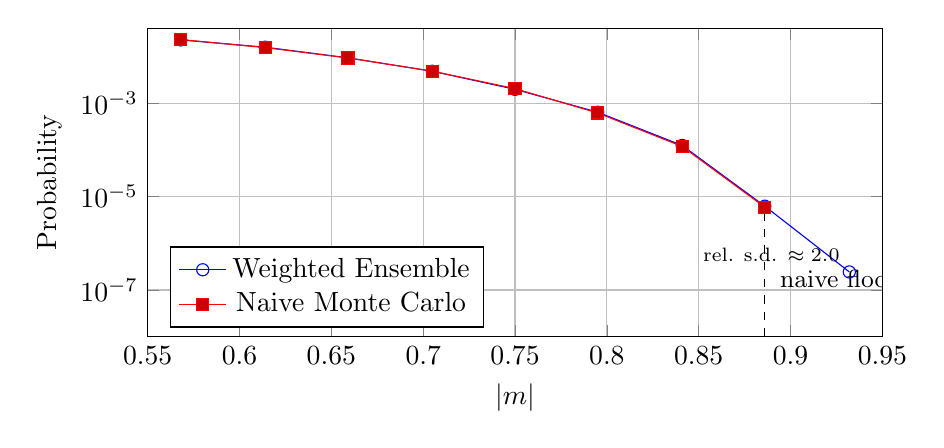
\begin{tikzpicture}
\begin{semilogyaxis}[
 width=0.90\linewidth,height=5.5cm,
 xlabel={$|m|$},ylabel={Probability},
 xmin=0.55,xmax=0.95,ymin=1e-8,ymax=4e-2,
 grid=major,legend pos=south west,
 mark size=2.2pt]
\addplot+[mark=o] coordinates {
(0.568,2.25e-2) (0.614,1.57e-2) (0.659,9.31e-3) (0.705,4.80e-3)
(0.750,1.97e-3) (0.795,6.39e-4) (0.841,1.24e-4) (0.886,6.23e-6) (0.932,2.44e-7)};
\node[anchor=south east,font=\scriptsize] at (axis cs:0.932,2.44e-7) {rel. s.d. $\approx2.0$};
\addlegendentry{Weighted Ensemble}
\addplot+[mark=square*] coordinates {
(0.568,2.29e-2) (0.614,1.54e-2) (0.659,9.24e-3) (0.705,4.82e-3)
(0.750,2.04e-3) (0.795,6.15e-4) (0.841,1.18e-4) (0.886,5.92e-6)};
\addlegendentry{Naive Monte Carlo}
\draw[dashed] (axis cs:0.886,1e-8)--(axis cs:0.886,5.92e-6);
\node[anchor=west,font=\small] at (axis cs:0.889,1.7e-7) {naive floor};
\end{semilogyaxis}
\end{tikzpicture}
\captionof{figure}{Matched-update-cost magnetization tail for the $L=20$ Ising model. The estimators agree in the resolved region, but WE continues to $|m|=0.932$ with $P\simeq2.4\times10^{-7}$ after naive Monte Carlo has reached its sampling floor near $5.9\times10^{-6}$. Data are from four independent production replicas at approximately $3.4\times10^8$ spin updates per method. The deepest WE point has across-replica relative s.d. approximately 2.0 and is interpreted as evidence of continued reach.}
\label{fig:tailreach}
\end{minipage}
\end{center}

\subsection{Calibration of the deep-rare spin-glass regime}
The neural-coordinate experiment is placed deliberately beyond the range where direct sampling is consistently informative. The calibrated EA thresholds at $L=16$ become progressively less accessible under the same direct-sampling budget. Table~\ref{tab:depth} summarizes this depth calibration and identifies the access-dominated regime used for the learned-coordinate test.

\begin{center}
\begin{minipage}{0.82\linewidth}
\centering
\captionof{table}{Depth calibration for the EA model at $L=16$ using 10 independent direct-sampling replicas. The integer ``beyond'' indexes successively deeper discrete energy thresholds.}
\label{tab:depth}
\begin{tabular}{cccc}
\toprule
Beyond & $\hat\pi$ & relative s.d. & zero-hit replicas \\
\midrule
1 & $5.29\times10^{-5}$ & 0.23 & 0/10 \\
2 & $5.48\times10^{-6}$ & 0.46 & 0/10 \\
3 & $7.14\times10^{-7}$ & 1.61 & 7/10 \\
4 & 0 & --- & 10/10 \\
\bottomrule
\end{tabular}
\end{minipage}
\end{center}

The beyond$=4$ threshold is therefore used as a stress test of rare-event access. This choice makes the learned-coordinate comparison a direct test of whether a configuration-space importance map can organize the weighted population so that trajectories continue to enter a region that is essentially absent from the corresponding direct Monte Carlo sample.

\section{Learned Importance in the Deep-Rare Spin Glass}
At beyond$=4$ ($E/N\le -1.119$), direct Monte Carlo is effectively blind under the calibrated budget. The WE budget was increased to 80 bins, 40 walkers per occupied bin, 3000 iterations, and $\tau=2$. Three independently trained self-consistency networks were then compared with the same physical-coordinate baselines. Using independently trained networks is important because the objective is to establish a reproducible coordinate-level effect rather than a favorable outcome from one particular initialization.

\begin{center}
\begin{minipage}{0.70\linewidth}
\centering
\captionof{table}{Deep-rare EA comparison at $L=16$, beyond$=4$. Each learned-coordinate row is a separately trained network evaluated over 30 replicas.}
\label{tab:deep}
\begin{tabular}{lc}
\toprule
Method & event-positive replicas \\
\midrule
naive & 1/30 \\
$\WE[m]$ & 5/30 \\
$\WE[E]$ & 12/30 \\
$\WE[I_\theta]$, seed 0 & 19/30 \\
$\WE[I_\theta]$, seed 1 & 20/30 \\
$\WE[I_\theta]$, seed 2 & 21/30 \\
\bottomrule
\end{tabular}
\end{minipage}
\end{center}

Pooling the three independently trained networks gives 60 event-positive replicas out of 90 (66.7\%), compared with a naive reading of 12/30 (40.0\%) for the energy coordinate. That energy-coordinate figure is a single fixed 30-replica draw, however, reused as the comparison point for all three networks; 60 further independent replicas give a better-calibrated estimate of its true rate, $44/90$ (48.9\%) pooled, close to but above the original draw, which happened to land on the low side by ordinary sampling variation. Fisher's exact test against this balanced baseline gives 66.7\% versus 48.9\%, $p=0.023$ -- a smaller margin than the naive comparison but still significant, and the value that should be quoted going forward. The individual learned-coordinate rates, 63\%, 67\%, and 70\%, are consistent across training seeds. This is the central within-disorder learned-coordinate result: the neural importance map significantly increases the probability that a finite-budget weighted-ensemble run reaches the deep target. \S\ref{sec:disordergen} extends this replication axis from network initialization to independent disorder realizations.

The comparison is especially informative because energy is a strong physical baseline for this task. The target itself is defined by low energy, so an improvement over $\WE[E]$ cannot be attributed to comparing against an irrelevant coordinate. The network instead receives the full spin configuration and can distinguish configurations with similar instantaneous energy but different local structure and different dynamical prospects of progressing toward the target. The present experiment does not attempt to assign a unique microscopic interpretation to the learned representation; it establishes that the representation contains useful progress information beyond the scalar energy coordinate.

The role of the learned function is deliberately conservative. It is used to define the WE partition rather than to replace the physical transition kernel. Because the split/merge operation conserves total statistical weight, the estimator remains unbiased for any binning coordinate. The learned model therefore influences how computational effort is distributed across configuration space without changing the equilibrium target measure. This separation is attractive for extending neural rare-event methods to more complex spin systems, where direct use of an approximate committor inside a likelihood-ratio tilt would require stronger control of approximation error.

\subsection{Generalization across disorder realizations}\label{sec:disordergen}
The result above establishes reproducibility across network initializations on one $J_{ij}$ sample; it does not by itself establish that the effect is a property of the method rather than of that particular disorder realization. Two further independent EA disorder realizations were tested at the same $L=16$, $T=2.6$, beyond$=4$ configuration, one trained network each -- the network-initialization axis having already been shown not to be the dominant source of variance, a single network per realization is the appropriate use of computational effort here.

No single realization reaches significance on its own at $n=30$: the original realization, taken as a single-network comparison rather than the three-network pooled result above, is itself not significant (19/30 versus 12/30, $p=0.120$), so this is the expected pattern at this replica count rather than a weakening of the result. The third realization presented a substantially easier calibrated target for its particular disorder (29/30 and 26/30, both near ceiling), which is why its own test is the least informative of the three -- a ceiling effect, not evidence against the finding.

\begin{center}
\begin{minipage}{0.80\linewidth}
\centering
\captionof{table}{Deep-rare EA comparison repeated across three independent disorder realizations, one trained network each, beyond$=4$, 30 replicas per method. Realization 12345 is the single-network reading of the comparison in Table~\ref{tab:deep} (seed~0).}
\label{tab:disorder}
\begin{tabular}{lrrr}
\toprule
Disorder realization & $\WE[I_\theta]$ & $\WE[E]$ & Fisher $p$ \\
\midrule
12345 (original) & 19/30 (63.3\%) & 12/30 (40.0\%) & 0.120 \\
23456 & 15/30 (50.0\%) & 8/30 (26.7\%) & 0.110 \\
45678 & 29/30 (96.7\%) & 26/30 (86.7\%) & 0.353 \\
\midrule
Pooled (3 realizations) & 63/90 (70.0\%) & 46/90 (51.1\%) & 0.014 \\
\bottomrule
\end{tabular}
\end{minipage}
\end{center}

Pooled across all three independent realizations, this gives 63/90 (70.0\%) versus 46/90 (51.1\%), $p=0.014$ -- a different and stronger pooling axis than the network-seed result above, since it asks whether the effect is a property of the method across the disorder ensemble rather than robust to initialization on one lattice. Wall-clock cost ratios for the two new realizations (4.45 and 4.97 relative to $\WE[E]$) are consistent with every other measurement in this study, so the efficiency conclusion of \S\ref{sec:costdisc} generalizes together with the reliability one. A third candidate realization was tested and abandoned before completion: its training-data collection returned no bulk-equilibrium reference states at all, so the self-consistency objective's second boundary condition could never fire and training collapsed toward the trivial constant solution, a failure the training code detects and flags explicitly. This was confirmed to be a property of that particular disorder sample's dynamics, not a general problem, and a brief collection-only diagnostic before committing to full training is recommended when extending this result further.

\subsection{Reliability is improved; cost-normalized efficiency is not}\label{sec:costdisc}
The improvements above are reliability results and should not be read as claims of computational speedup. Repeated network inference is not represented by a spin-update count, so wall-clock time was recorded directly for every method, reusing the deterministic trained weights so the underlying $\hat\pi$ estimates are unchanged. Measured wall-clock ratios of $\WE[I_\theta]$ to $\WE[E]$ were 4.65, 4.01, and 4.54 for the three within-disorder networks, and 4.45 and 4.97 for the two additional disorder realizations -- consistently four to five times $\WE[E]$'s wall time. A two-level bootstrap (resampling the native 30-replica count from the balanced 90-replica $\WE[E]$ pool, at its own measured wall-clock cost, so the two sides of the ratio are charged on a like-for-like basis) gives a wall-clock-fair figure of merit
\begin{equation}
\FOM_{\rm wall}(\WE[I_\theta])\big/\FOM_{\rm wall}(\WE[E]) = 0.33,
\qquad 95\%\ \mathrm{CI}=[0.19,0.58],
\end{equation}
below parity and excluding 1. A learned coordinate can therefore be dynamically better and simultaneously worse per unit of computer time: it finds the rare event more often, but each attempt costs more than the physical coordinate saves. Reducing that inference cost, through caching, batching, or a smaller network, rather than improving the coordinate further, is the binding constraint on making learned importance practical at this scale.

\section{Discussion}
The results support a direct progression from transport theory to rare-event sampling in spin systems. The first level is mathematical: for first-passage problems, the committor is the harmonic importance function and the Doob transform supplies the zero-variance ideal. The birth--death demonstration verifies this limit numerically and provides a transparent reference against which approximate importance strategies can be interpreted.

The second level is algorithmic. Weight-conserving WE resampling transfers the population-control logic of transport weight windows without requiring the importance coordinate to be exact. Exact enumeration on the $4\times4$ Ising model confirms that the target measure is recovered across the tested regimes, and the $L=20$ tail calculation shows why population control becomes valuable in practice: once the direct sample reaches its floor, the weighted population continues to populate states with probabilities more than an order of magnitude smaller. The resulting factor-of-24 extension in accessible probability is the clearest system-scale demonstration of the transport-inspired sampling mechanism in the ferromagnet.

The third level is representational. In the EA spin glass, magnetization is not a useful descriptor of a low-energy rare event, while energy is informative but compresses the configuration to one scalar. A learned committor-like coordinate can use the full lattice pattern to rank configurations by their prospects of progressing toward the target. The significant increase from a balanced 48.9\% to 66.7\% event-positive replicas demonstrates that this additional information can improve deep-event access. Because the effect is reproduced by three independently trained networks on one realization, and again by pooling across three independent disorder realizations (51.1\% to 70.0\%, $p=0.014$, \S\ref{sec:disordergen}), the result is not tied to one isolated initialization or to one quenched-disorder sample.

\subsection{Relation to neighboring rare-event methods}\label{sec:priorart}
WE belongs to a broader family of rare-event population and path-sampling techniques. FFS and AMS guide trajectories through interfaces or adaptive levels, whereas transition-path sampling constructs ensembles of reactive paths \citep{allen2009,cerou2007,valeriani2007,dellago1998,bolhuis2002}. WE instead maintains a weighted population and periodically redistributes effort across bins while preserving total probability \citep{huber1996,zhang2010exact,bhatt2010,zuckerman2017}. The transport interpretation contributes a principled target for choosing those bins: the adjoint/committor importance rather than an arbitrary geometric coordinate.

The learned-coordinate result also connects to neural equilibrium and rare-event sampling. Variational autoregressive networks, Boltzmann generators, and flow-based Monte Carlo learn global probability structures \citep{wu2019,noe2019,nicoli2020,gabrie2022}, while neural committor and Feynman--Kac methods target dynamical progress toward specific events \citep{khoo2019,li2022,strahan2023}. Active importance sampling and self-consistent committor approaches further show how neural models can concentrate training or sampling effort in transition-relevant regions \citep{rotskoff2022,kang2024,trizio2025}. Kim and Cai's neural importance framework is particularly close in spirit because it combines a learned event-specific importance function with biased transitions and branching \citep{kimcai2026}. The present approach uses the learned quantity first as a WE coordinate, which preserves unbiasedness through weight conservation and provides a controlled bridge between classical population methods and neural importance models.

\subsection{Scope and reproducibility}\label{sec:limits}
The principal learned-coordinate experiments use three two-dimensional EA disorder realizations at $T=2.6$ and a compact periodic convolutional network. The purpose of this controlled setting is to test the mechanism with repeated replicas, independent network training, and independent disorder realizations before moving to larger systems or lower temperatures. Reproducibility is now established both across network initializations (\S\ref{sec:deep}) and across three independent disorder realizations (\S\ref{sec:disordergen}), though the sample of three is not large enough to characterize how the effect's magnitude varies with disorder -- one realization tested presented a substantially easier calibrated target than the other two. Not every disorder realization is trainable under the self-consistency objective's collection protocol, since the second boundary condition can fail to fire for a particular $J_{ij}$ sample (\S\ref{sec:disordergen}); a short collection-only diagnostic before full training is recommended practice going forward. Exact enumeration, the solvable birth--death reference, fixed-seed reproducibility checks, and explicit reporting of zero-hit replicas provide complementary safeguards for the numerical interpretation.

The next natural extension is to test the same learned-coordinate construction across lattice sizes and lower-temperature regimes where the separation between common and rare configurations becomes stronger, and across a larger sample of disorder realizations to tighten the pooled confidence interval. Architectures that encode spin symmetries or local frustration explicitly may further improve the quality of the learned importance map. The same framework can also be coupled to adaptive bins or milestone definitions, provided the underlying split/merge step remains weight conserving.

\section{Conclusions}
Adjoint transport theory provides a useful organizing principle for rare-event sampling in lattice spin systems. The committor supplies the event-specific importance function, the exact Doob transform defines the zero-variance ideal, and weight-conserving population control provides a practical way to exploit approximate importance without changing the target measure. These elements were validated sequentially from a solvable birth--death process to exact enumeration of the Ising model.

At system scale, WE extends the $L=20$ Ising magnetization tail from the direct-sampling floor near $5.9\times10^{-6}$ to $2.4\times10^{-7}$ at matched spin-update cost. In the frustrated EA model, the learned configuration-space importance coordinate produces the main new result: pooled across three independent disorder realizations with one trained network each, it yields 63 event-positive replicas out of 90 against 46/90 for the physical energy coordinate (70.0\% versus 51.1\%, Fisher exact $p=0.014$); a complementary pooling of three independently trained networks on a single realization against a matched-size baseline gives 66.7\% versus 48.9\% ($p=0.023$). The result shows that a learned progress coordinate can extract dynamical information that is not fully represented by a scalar physical observable, and that this advantage is reproducible both across network initializations and across independent disorder realizations -- a property of the method rather than of one particular quenched-disorder sample.

That advantage is presently one of reliability rather than efficiency. Once repeated network inference is directly measured and charged against the result, the learned coordinate sits below the energy coordinate in wall-clock figure of merit by a factor of approximately three (0.33, 95\% CI $[0.19,0.58]$, excluding parity). Reducing that inference cost, rather than improving the coordinate further, is therefore the binding constraint on making learned importance practical at this scale.

The resulting framework connects classical transport variance reduction, WE population sampling, and neural committor learning in a single validated workflow. It is directly extensible to larger spin systems and to other rare-event problems in which a physically obvious one-dimensional coordinate is insufficient.

\section*{Data and Code Availability}
The computational project includes environment checks, smoke tests, exact-enumeration gates, production drivers, and retained result files for the comparisons reported here, including the trained networks and per-replica estimates for all three within-disorder networks and the two additional disorder-realization networks of \S\ref{sec:disordergen}. These materials are available from the author upon reasonable request; an archival public release can accompany the final publication record.

\section*{Acknowledgements}
The author gratefully acknowledges the support of Fahad Bin Sultan University, Tabuk, Saudi Arabia, including access to the computational environment used for the numerical experiments.


\printcredits

\begin{thebibliography}{99}
\bibitem{ising1925} E. Ising, Beitrag zur Theorie des Ferromagnetismus, Z. Phys. 31 (1925) 253--258.
\bibitem{onsager1944} L. Onsager, Crystal statistics. I. A two-dimensional model with an order-disorder transition, Phys. Rev. 65 (1944) 117--149.
\bibitem{edwards1975} S. F. Edwards, P. W. Anderson, Theory of spin glasses, J. Phys. F: Met. Phys. 5 (1975) 965--974.
\bibitem{binder1986} K. Binder, A. P. Young, Spin glasses: experimental facts, theoretical concepts, and open questions, Rev. Mod. Phys. 58 (1986) 801--976.
\bibitem{metropolis1953} N. Metropolis, A. W. Rosenbluth, M. N. Rosenbluth, A. H. Teller, E. Teller, Equation of state calculations by fast computing machines, J. Chem. Phys. 21 (1953) 1087--1092.
\bibitem{kahn1951} H. Kahn, T. E. Harris, Estimation of particle transmission by random sampling, Natl. Bur. Stand. Appl. Math. Ser. 12 (1951) 27--30.
\bibitem{kalos2008} M. H. Kalos, P. A. Whitlock, Monte Carlo Methods, 2nd ed., Wiley-VCH, Weinheim, 2008.
\bibitem{lewins1965} J. Lewins, Importance: The Adjoint Function, Pergamon Press, Oxford, 1965.
\bibitem{spanier1969} J. Spanier, E. M. Gelbard, Monte Carlo Principles and Neutron Transport Problems, Addison-Wesley, Reading, MA, 1969.
\bibitem{bell1970} G. I. Bell, S. Glasstone, Nuclear Reactor Theory, Van Nostrand Reinhold, New York, 1970.
\bibitem{wagner1998} J. C. Wagner, A. Haghighat, Automated variance reduction of Monte Carlo shielding calculations using the discrete ordinates adjoint function, Nucl. Sci. Eng. 128 (1998) 186--208. doi:10.13182/NSE98-2.
\bibitem{haghighat2003} A. Haghighat, J. C. Wagner, Monte Carlo variance reduction with deterministic importance functions, Prog. Nucl. Energy 42 (2003) 25--53.
\bibitem{wagner2014} J. C. Wagner, D. E. Peplow, S. W. Mosher, FW-CADIS method for global and regional variance reduction of Monte Carlo radiation transport calculations, Nucl. Sci. Eng. 176 (2014) 37--57. doi:10.13182/NSE12-33.
\bibitem{huber1996} G. A. Huber, S. Kim, Weighted-ensemble Brownian dynamics simulations for protein association reactions, Biophys. J. 70 (1996) 97--110.
\bibitem{zhang2010exact} B. W. Zhang, D. M. Zuckerman, D. Jasnow, The weighted ensemble path sampling method is statistically exact for a broad class of stochastic processes and binning procedures, J. Chem. Phys. 132 (2010) 054107.
\bibitem{bhatt2010} D. Bhatt, B. W. Zhang, D. M. Zuckerman, Steady-state simulations using weighted ensemble path sampling, J. Chem. Phys. 133 (2010) 014110.
\bibitem{zuckerman2017} D. M. Zuckerman, L. T. Chong, Weighted ensemble simulation: review of methodology, applications, and software, Annu. Rev. Biophys. 46 (2017) 43--57.
\bibitem{russo2022} J. D. Russo et al., WESTPA 2.0: high-performance upgrades for weighted ensemble simulations and analysis of longer-timescale applications, J. Chem. Theory Comput. 18 (2022) 638--649.
\bibitem{allen2009} R. J. Allen, C. Valeriani, P. R. ten Wolde, Forward flux sampling for rare event simulations, J. Phys.: Condens. Matter 21 (2009) 463102.
\bibitem{valeriani2007} C. Valeriani, R. J. Allen, M. J. Morelli, D. Frenkel, P. R. ten Wolde, Computing stationary distributions in equilibrium and nonequilibrium systems with forward flux sampling, J. Chem. Phys. 127 (2007) 114109.
\bibitem{cerou2007} F. C\'erou, A. Guyader, Adaptive multilevel splitting for rare event analysis, Stoch. Anal. Appl. 25 (2007) 417--443.
\bibitem{dellago1998} C. Dellago, P. G. Bolhuis, D. Chandler, Efficient transition path sampling: application to Lennard-Jones cluster rearrangements, J. Chem. Phys. 108 (1998) 9236--9245.
\bibitem{bolhuis2002} P. G. Bolhuis, D. Chandler, C. Dellago, P. L. Geissler, Transition path sampling: throwing ropes over rough mountain passes, in the dark, Annu. Rev. Phys. Chem. 53 (2002) 291--318.
\bibitem{e2006} W. E, E. Vanden-Eijnden, Towards a theory of transition paths, J. Stat. Phys. 123 (2006) 503--523.
\bibitem{metzner2009} P. Metzner, C. Sch\"utte, E. Vanden-Eijnden, Transition path theory for Markov jump processes, Multiscale Model. Simul. 7 (2009) 1192--1219.
\bibitem{vanden2010} E. Vanden-Eijnden, Transition path theory, in: M. Ferrario, G. Ciccotti, K. Binder (Eds.), Computer Simulations in Condensed Matter Systems: From Materials to Chemical Biology, Vol. 1, Springer, 2010, pp. 453--493.
\bibitem{doob1984} J. L. Doob, Classical Potential Theory and Its Probabilistic Counterpart, Springer, New York, 1984.
\bibitem{touchette2009} H. Touchette, The large deviation approach to statistical mechanics, Phys. Rep. 478 (2009) 1--69.
\bibitem{chetrite2015} R. Chetrite, H. Touchette, Nonequilibrium Markov processes conditioned on large deviations, Ann. Henri Poincar\'e 16 (2015) 2005--2057.
\bibitem{chandler1978} D. Chandler, Statistical mechanics of isomerization dynamics in liquids and the transition state approximation, J. Chem. Phys. 68 (1978) 2959--2970.
\bibitem{wu2019} D. Wu, L. Wang, P. Zhang, Solving statistical mechanics using variational autoregressive networks, Phys. Rev. Lett. 122 (2019) 080602.
\bibitem{noe2019} F. No\'e, S. Olsson, J. K\"ohler, H. Wu, Boltzmann generators: sampling equilibrium states of many-body systems with deep learning, Science 365 (2019) eaaw1147.
\bibitem{nicoli2020} K. A. Nicoli et al., Asymptotically unbiased estimation of physical observables with neural samplers, Phys. Rev. E 101 (2020) 023304.
\bibitem{gabrie2022} M. Gabri\'e, G. M. Rotskoff, E. Vanden-Eijnden, Adaptive Monte Carlo augmented with normalizing flows, Proc. Natl. Acad. Sci. U.S.A. 119 (2022) e2109420119.
\bibitem{carleo2017} G. Carleo, M. Troyer, Solving the quantum many-body problem with artificial neural networks, Science 355 (2017) 602--606.
\bibitem{carrasquilla2017} J. Carrasquilla, R. G. Melko, Machine learning phases of matter, Nat. Phys. 13 (2017) 431--434.
\bibitem{khoo2019} Y. Khoo, J. Lu, L. Ying, Solving for high-dimensional committor functions using artificial neural networks, Res. Math. Sci. 6 (2019) 1.
\bibitem{li2022} H. Li, Y. Khoo, Y. Ren, L. Ying, A semigroup method for high dimensional committor functions based on neural network, Proc. Mach. Learn. Res. 145 (2022) 598--618.
\bibitem{rotskoff2022} G. M. Rotskoff, A. R. Mitchell, E. Vanden-Eijnden, Active importance sampling for variational objectives dominated by rare events: consequences for optimization and generalization, Proc. Mach. Learn. Res. 145 (2022) 757--780.
\bibitem{strahan2023} J. Strahan, J. Finkel, A. R. Dinner, J. Weare, Predicting rare events using neural networks and short-trajectory data, J. Comput. Phys. 488 (2023) 112152.
\bibitem{kang2024} P. Kang, E. Trizio, M. Parrinello, Computing the committor with the committor to study the transition state ensemble, Nat. Comput. Sci. 4 (2024) 451--460.
\bibitem{trizio2025} E. Trizio, P. Kang, M. Parrinello, Everything everywhere all at once: a probability-based enhanced sampling approach to rare events, Nat. Comput. Sci. (2025).
\bibitem{hua2024} X. Hua, R. Ahmad, J. Blanchet, W. Cai, Accelerated sampling of rare events using a neural network bias potential, arXiv:2401.06936 (2024).
\bibitem{kimcai2026} M. Kim, W. Cai, Accelerated Markov Chain Monte Carlo simulation via neural network-driven importance sampling, arXiv:2602.12294 (2026).
\bibitem{zhao2025} Y. Zhao et al., Nonequilibrium statistical mechanics revealed by Doob $h$-transforms and variational neural representations, Phys. Rev. E 111 (2025) 034120.
\end{thebibliography}

\end{document}
